\documentclass[12pt,]{article}
\usepackage[utf8]{inputenc}
\usepackage[T1]{fontenc}
\usepackage{mathptmx}
\usepackage{geometry}
\usepackage{mathtools}
\usepackage[english]{babel}
\usepackage{graphicx}
\usepackage{stackengine}
\usepackage[os=win]{menukeys}
\usepackage{hyperref}
\usepackage{minted}
\usepackage{xcolor}
\usepackage{tikz}
\usepackage[yyyymmdd,hhmmss]{datetime}
\usepackage{etoolbox}
\usepackage[inline]{enumitem}

\newcommand{\WindowsLogo}{\raisebox{-0.1em}{
\includegraphics[height=0.8em]{images/logo/Windows_3_logo_simplified}}}
%\newcommand{\PowerLogo}{\raisebox{-0.1em}{
\includegraphics[height=0.8em]{images/logo/power}}}
\newcommand{\WinKey}{\keys{\WindowsLogo}}	
\newcommand{\PowerKey}{\keys{\PowerLogo}}	

\patchcmd{\thebibliography}{\section*{\refname}}{}{}{}

\newcommand{\ShowOsVersion}{
	\immediate\write18{\unexpanded{foo=`uname -sro` && echo "${foo}" > tmp.tex}}
	\input{tmp}\immediate\write18{rm tmp.tex}
}

\newcommand{\ShowTexVersion}{
	\immediate\write18{\unexpanded{foo=`pdflatex -version | head -n1 | cut -d' ' -f1,2` && echo "${foo}" > tmp.tex}}
	\input{tmp}\immediate\write18{rm tmp.tex}
}

\addto\captionsenglish{\renewcommand{\contentsname}{Daftar Isi}}
\addto\captionsenglish{\renewcommand{\figurename}{Gambar}}

\hypersetup{
	colorlinks=true, %set true if you want colored links
	linktoc=all,     %set to all if you want both sections and subsections linked
	linkcolor=blue,  %choose some color if you want links to stand out
	urlcolor=blue,	 %url color
}

\geometry{
	a4paper,
	left=15mm,
	right=10mm,
	top=10mm,
	bottom=15mm,
}

\title{\LARGE \bf
	Laporan Singkat\\
	\small{(Microcomputer Audiometri Prototype)}
}

\author{Achmadi ST MT}

\date{}

\hypersetup{citecolor=black}

\definecolor{LightGray}{gray}{0.95}

%\pagecolor[rgb]{0.1,0.1,0.1}
%\color[rgb]{1,1,1}

\begin{document}
	\thispagestyle{empty}
	
	\begin{titlepage}
		\centering
		\vfill
		\vfill
		\maketitle
		\vfill
		
\includegraphics[width=200pt]{images/logo/logoviblab}
		\vfill
		\vfill
		Update: {\today} \currenttime \\
	\end{titlepage}
	
	%%%%%%%%%%%%%%%%%%%%%%%%%%%%%%%%%%%%%%%%%%%%%%%%%%%%%%%%%%%%%%%%%
	
	\section{Setup}
	
	\subsection{Unit Prototype}
	
	Unit prototype terdiri atas:
	\begin{itemize}
		\item Raspberry-Pi versi 3-B
		\begin{figure}[!ht]
			\centering
			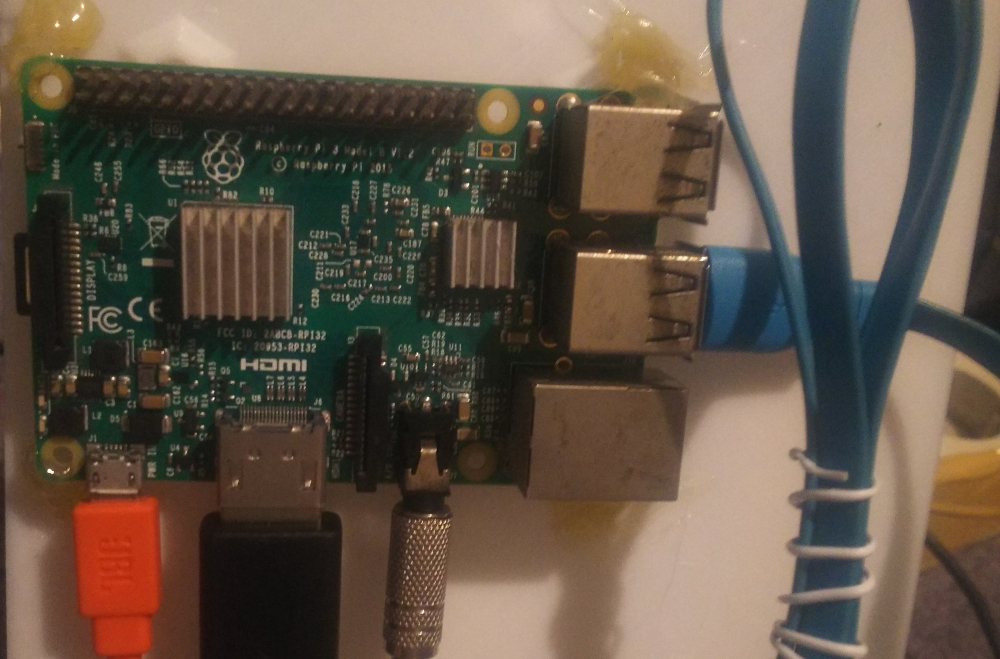
\includegraphics[width=250pt]{images/foto/raspi}
			\caption{RPi-3B}
		\end{figure}
		\item Waveshare LCD-TFT HDMI tipe C
		\begin{figure}[!ht]
			\centering
			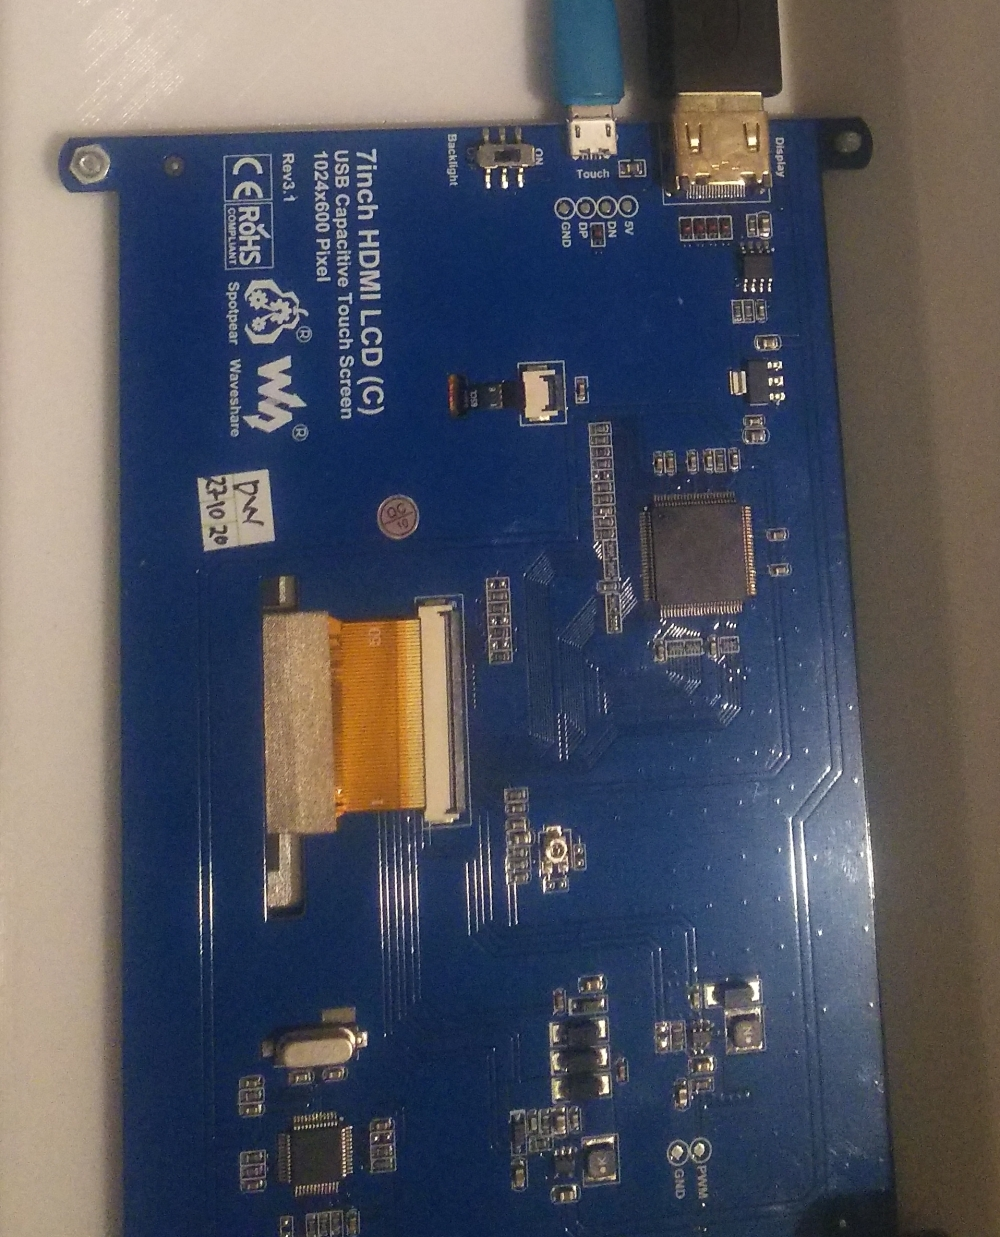
\includegraphics[width=200pt]{images/foto/lcd_back}
			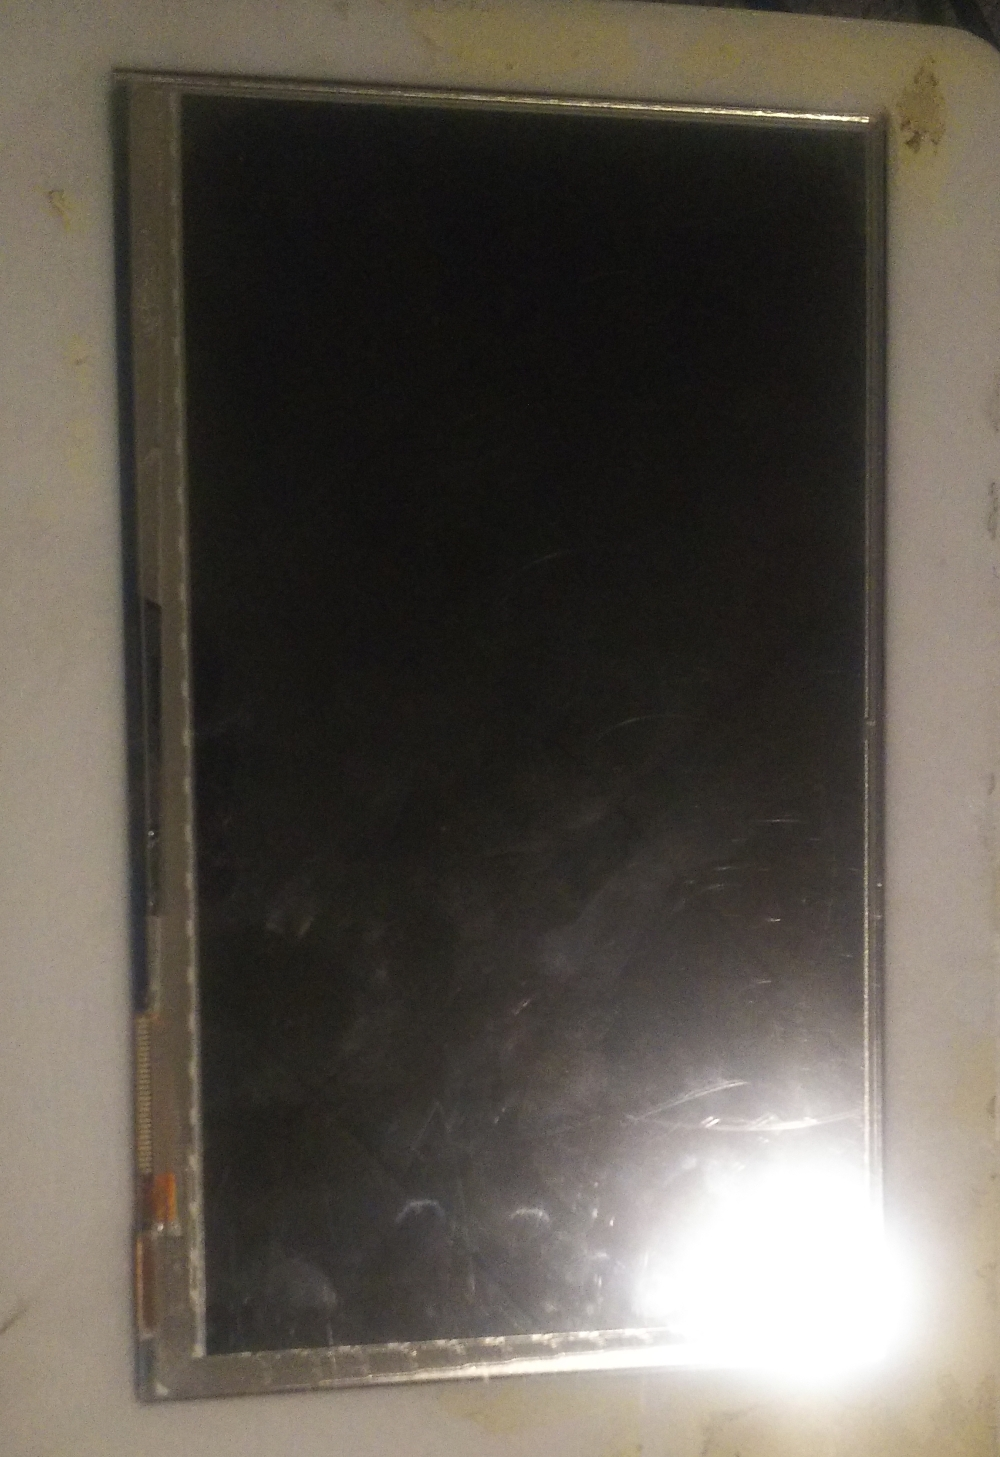
\includegraphics[width=200pt]{images/foto/lcd_front}
			\caption{LCD-TFT: (kiri) panel belakang dan (kanan) panel depan}
		\end{figure}
	\end{itemize}
	
	\newpage
	\subsection{Software}
	
	\subsubsection{Software Dasar}
	
	Software dasar yang digunakan adalah Pychoacoustics Lab yang \textit{source-tree} tersedia di:\\
	\url{https://github.com/sam81/pychoacoustics}
	
	Instalasi untuk Pacman-based Linux tersedia di:\\
	\url{https://github.com/mekatronik-achmadi/archmate-pkgbuild/tree/master/pychoacoustic}
	
	\begin{figure}[!ht]
		\centering
		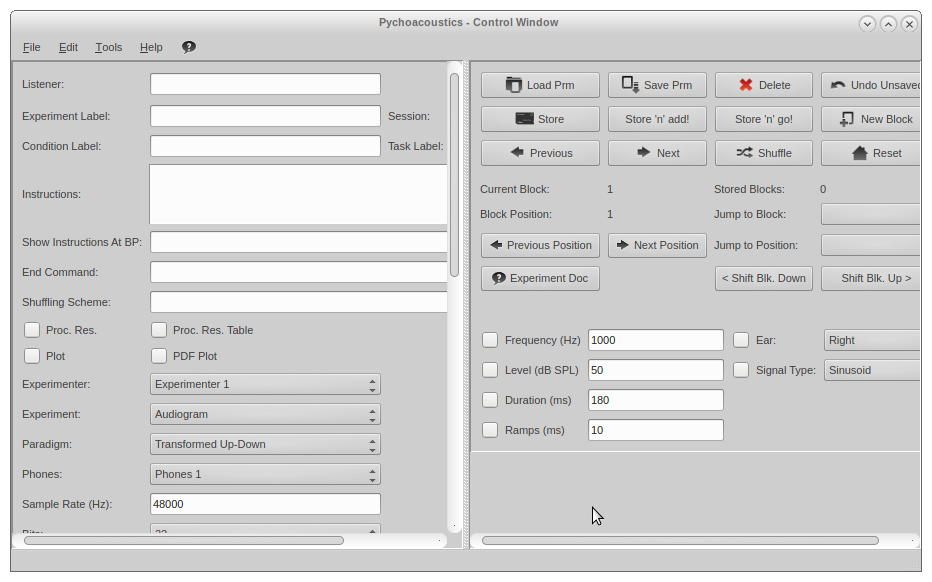
\includegraphics[width=250pt]{images/screen/piko}
		\caption{Pychoacoustics}
	\end{figure}

	\subsubsection{Software Uji}
	
	Untuk pengujian, digunakan dialog tone-generator yang menggunakan pustaka Python yang sama dengan software Pychoacoustics.
	
	Python Class dapat ditemukan di \url{https://github.com/VibrasticLab/pikoakustik/blob/stm32f401re_3pin/archlinuxarm/dialogPhones.py}.
	
	Dan skrip running dapat ditemukan di \url{https://github.com/VibrasticLab/pikoakustik/blob/stm32f401re_3pin/archlinuxarm/pychophone.py}
	
	\begin{figure}[!ht]
		\centering
		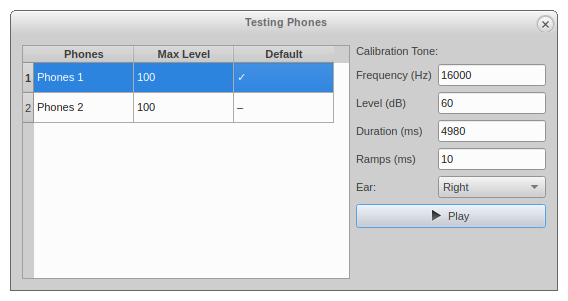
\includegraphics[width=250pt]{images/screen/phone}
		\caption{Dialog Tone-Generator}
	\end{figure}

	Pengaturan yang digunakan:
	\begin{itemize}
		\item Volume unit diatur maximal: Untuk sistem Linux yang menggunakan Pulseaudio-Alsa sebagai audio server, dapat menggunakan perintah:
		\begin{minted}[frame=lines,framesep=2mm,fontsize=\small]{text}
pactl set-default-sink alsa_output.platform-bcm2835_audio.stereo-fallback.2
pactl set-sink-volume @DEFAULT_SINK@ 100%
		\end{minted}
		
		\item Durasi 4980 ms. Sehingga dengan ditambah ramp di awal dan akhir sebesar 10ms, maka total menjadi 5 detik
		
		\item Frekuensi (dalam Hz) diurut mulai 250, 500, 1000, 2000, 4000, 8000, dan 16000.
		
		\item Level (dalam dB) untuk setiap frekuensi diurut mulai 90, 80, 70, 60, 50, 40, dan 30.
	\end{itemize}

	\newpage
	\subsection{Eksperimen}
	
	Berikut penjelasan setup eksperimen:
	
	\begin{itemize}
		\item Microphone yang digunakan adalah merek dBX.
		\item Headphone yang digunakan adalah Miniso dan BOSE.
		\begin{figure}[!ht]
			\centering
			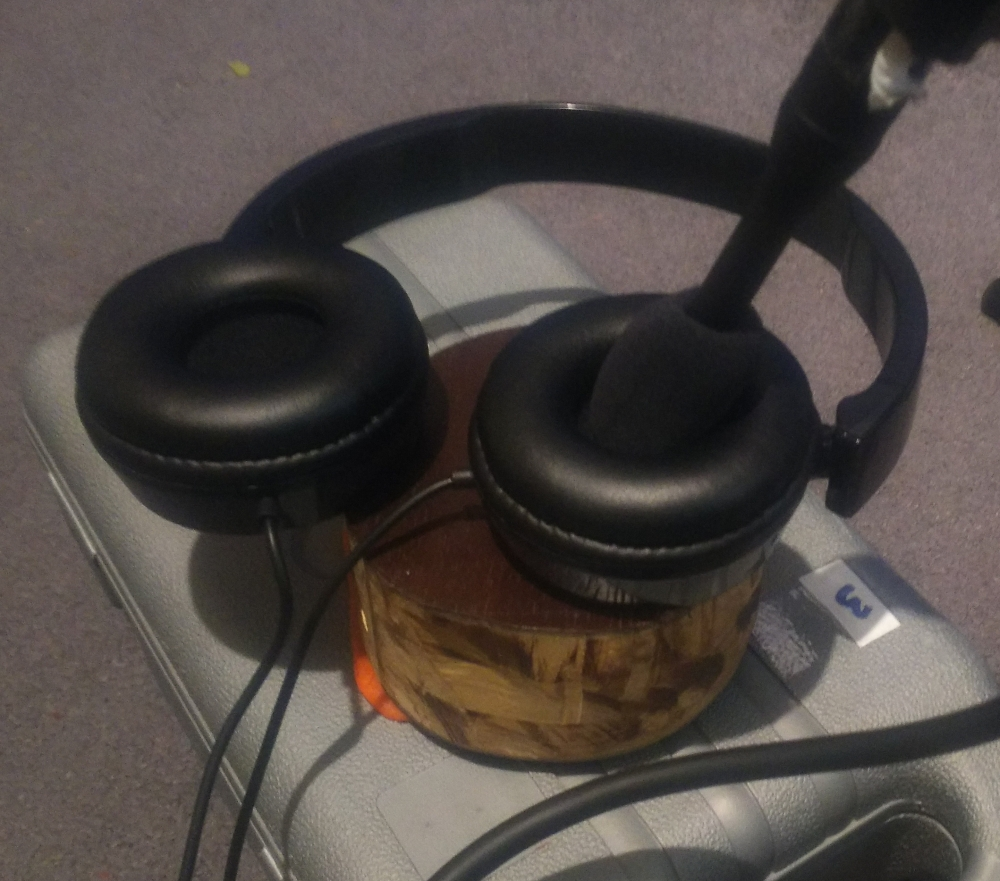
\includegraphics[width=200pt]{images/foto/miniso}
			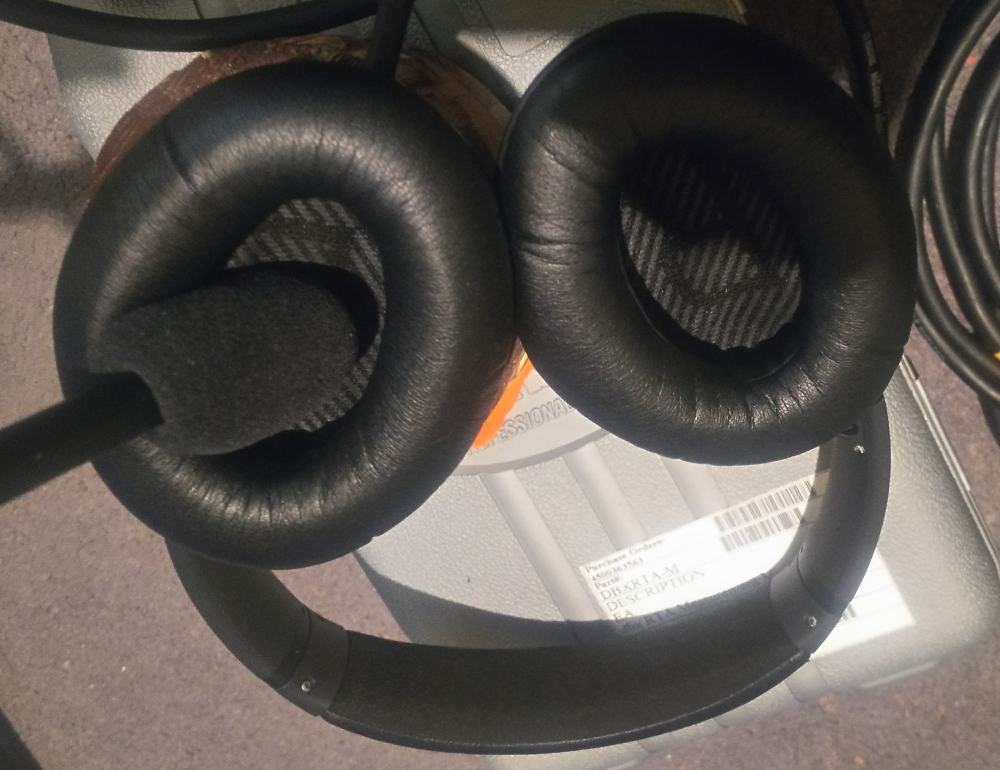
\includegraphics[width=200pt]{images/foto/bose}
			\caption{Headphone: (kiri) Miniso dan (kanan) BOSE}
		\end{figure}
		\item Audio Capture Device menggunakan Focusrite Scarlett 18i8.
		Input Gain diatur maximum.
		\begin{figure}[!ht]
			\centering
			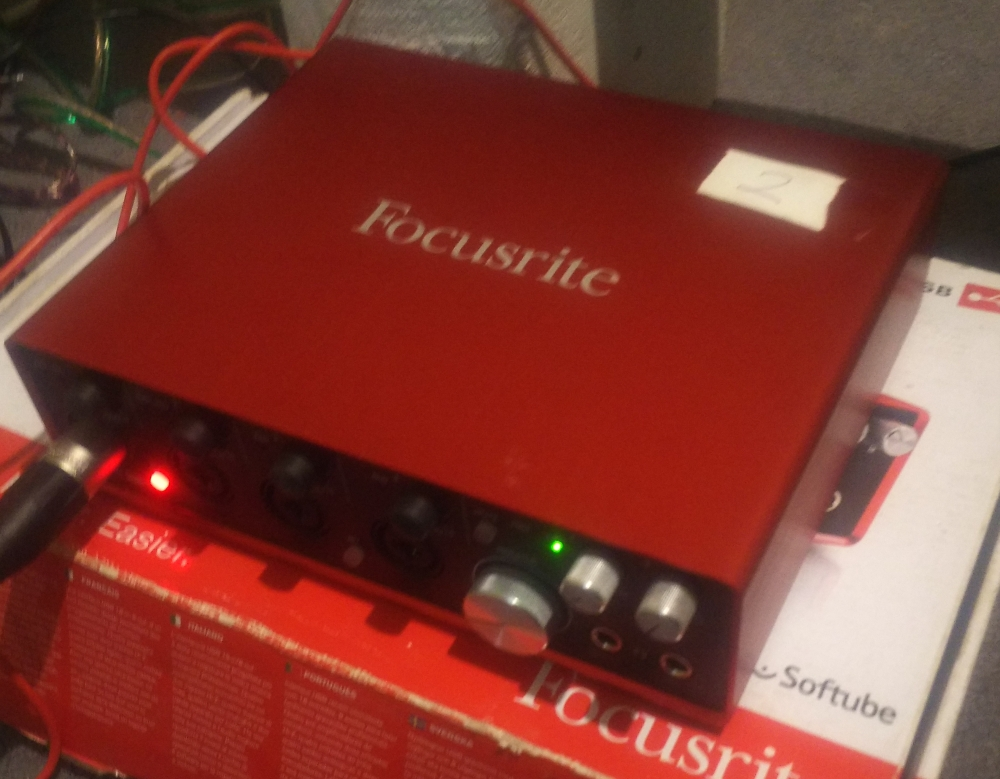
\includegraphics[width=200pt]{images/foto/capture}
			\caption{Scarlett 18i8}
		\end{figure}
	
		\item Software Capture menggunakan Real-Time Analyzer DSSF3 buatan Yoshimasha.
		Fungsi yang digunakan adalah FFT-Analyzer dengan A-weighting.
		
	\end{itemize}

	\subsection{Matrix Hasil yang diharapkan}
	
	Matrix hasil yang diharap dari hasil pengujian adalah nilai aktual (dalam SPL dB) sebagai berikut:
	
	\begin{center}
		\begin{tabular}{|c|c|c|c|c|c|c|c|} 
			\hline
			Fq/Ap & 90dB & 80dB & 70dB & 60dB & 50dB & 40dB & 30dB\\ [0.5ex] 
			\hline\hline
			250Hz & X dB & X dB & X dB & X dB & X dB & X dB & X dB \\
			\hline
			500Hz & X dB & X dB & X dB & X dB & X dB & X dB & X dB \\
			\hline
			1000Hz & X dB & X dB & X dB & X dB & X dB & X dB & X dB \\
			\hline
			2000Hz & X dB & X dB & X dB & X dB & X dB & X dB & X dB \\
			\hline
			4000Hz & X dB & X dB & X dB & X dB & X dB & X dB & X dB \\
			\hline
			8000Hz & X dB & X dB & X dB & X dB & X dB & X dB & X dB \\
			\hline
			16000Hz & X dB & X dB & X dB & X dB & X dB & X dB & X dB \\
			\hline
		\end{tabular}
	\end{center}

	\section{Hasil}
	
	\subsection{Ground Measurement}
	
	Berikut capture kondisi pengukuran tanpa \textit{tone-generation} apa pun:
	
	\begin{figure}[!ht]
		\centering
		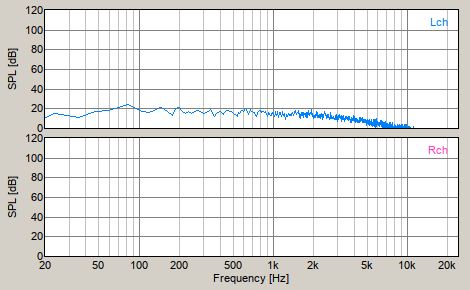
\includegraphics[width=300pt]{hasil_rpi/ground_Aweight}
		\caption{Ground Measurement}
	\end{figure}

	\newpage
	\subsection{Hasil Pengukuran}
	
	Berikut grafik yang ditarik dari file-file CSV hasil capture.
	Skrip Python untuk membuat grafiknya tersedia di \url{https://github.com/VibrasticLab/pikoakustik/tree/stm32f401re_3pin/document/short_test/hasil_rpi/python}
	
	\subsubsection{Miniso}
	
	Kumpulan CSV hasil pengukuran untuk headphone Miniso: \url{https://github.com/VibrasticLab/pikoakustik/tree/stm32f401re_3pin/document/short_test/hasil_rpi/miniso/}
	
	\begin{figure}[!ht]
		\centering
		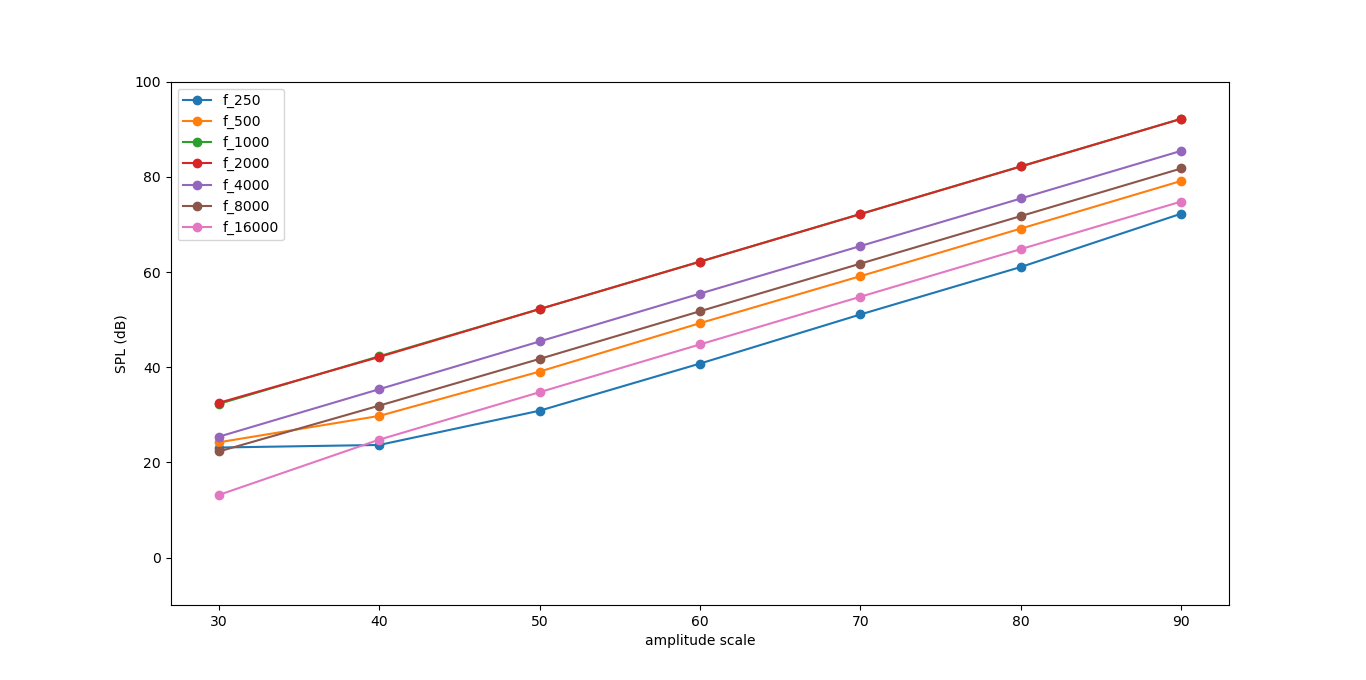
\includegraphics[width=450pt]{images/graph/miniso_each}
		\caption{Respon Aktual Level di setiap Frekuensi dan Level}
	\end{figure}

	\begin{figure}[!ht]
		\centering
		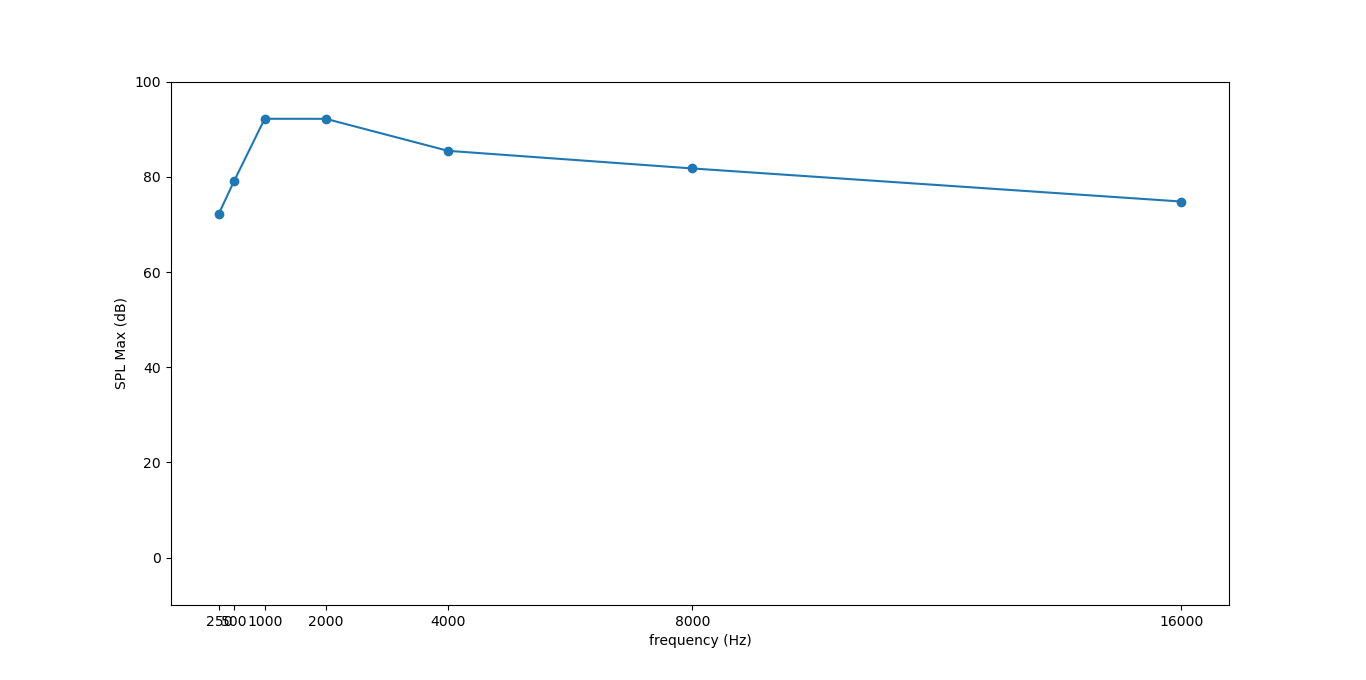
\includegraphics[width=450pt]{images/graph/miniso_allmax}
		\caption{Respon maximum Level di semua Frekuensi}
	\end{figure}

	\newpage
	\subsubsection{BOSE}
	Kumpulan CSV hasil pengukuran untuk headphone BOSE: \url{https://github.com/VibrasticLab/pikoakustik/tree/stm32f401re_3pin/document/short_test/hasil_rpi/bose/}
	
	\begin{figure}[!ht]
		\centering
		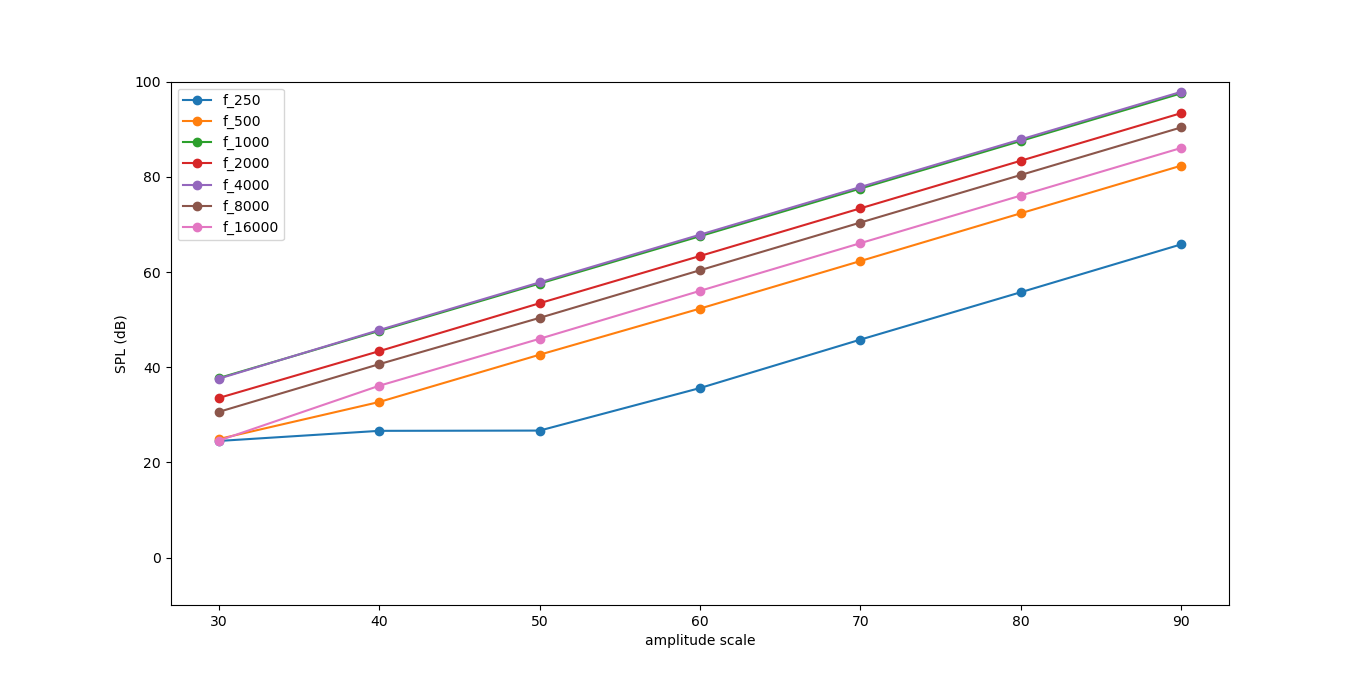
\includegraphics[width=450pt]{images/graph/bose_each}
		\caption{Respon Aktual Level di setiap Frekuensi dan Level}
	\end{figure}
	
	\begin{figure}[!ht]
		\centering
		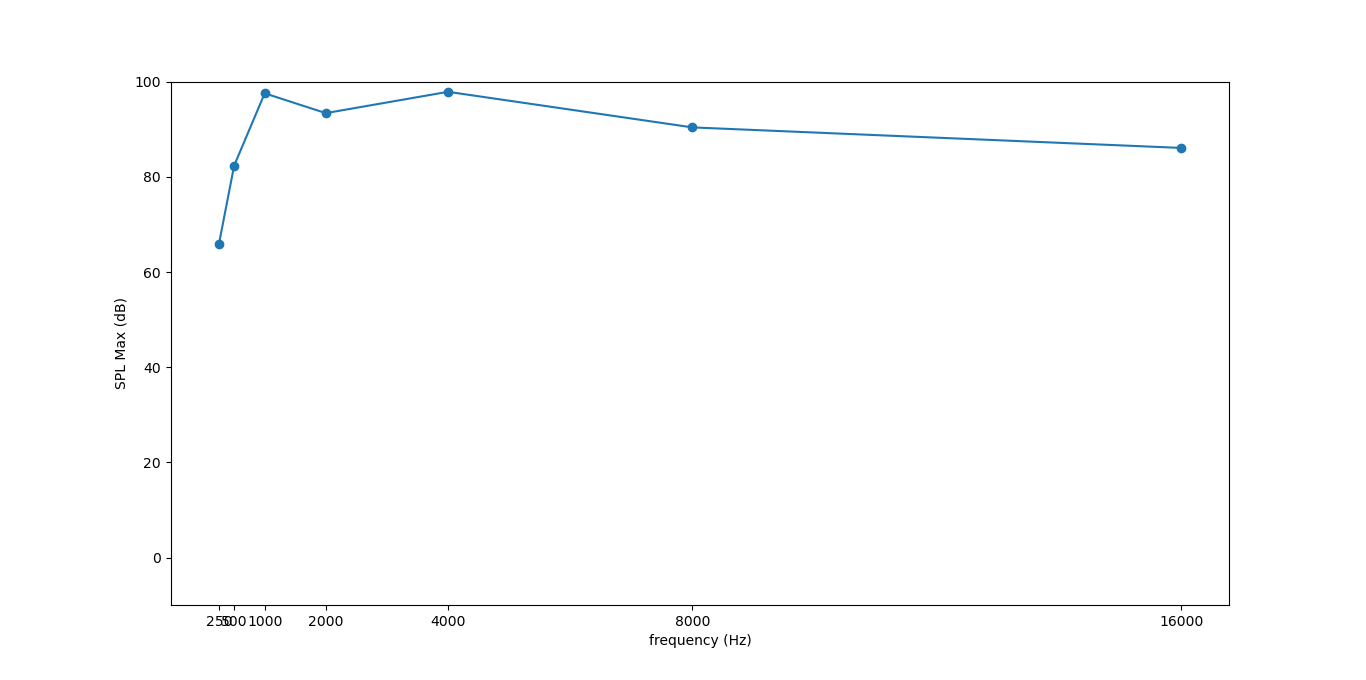
\includegraphics[width=450pt]{images/graph/bose_allmax}
		\caption{Respon maximum Level di semua Frekuensi}
	\end{figure}

	\newpage
	\subsubsection{Komparasi}
	
	Berikut grafik perbandingan level maximum di semua frekuensi untuk semua headphone.
	
	\begin{figure}[!ht]
		\centering
		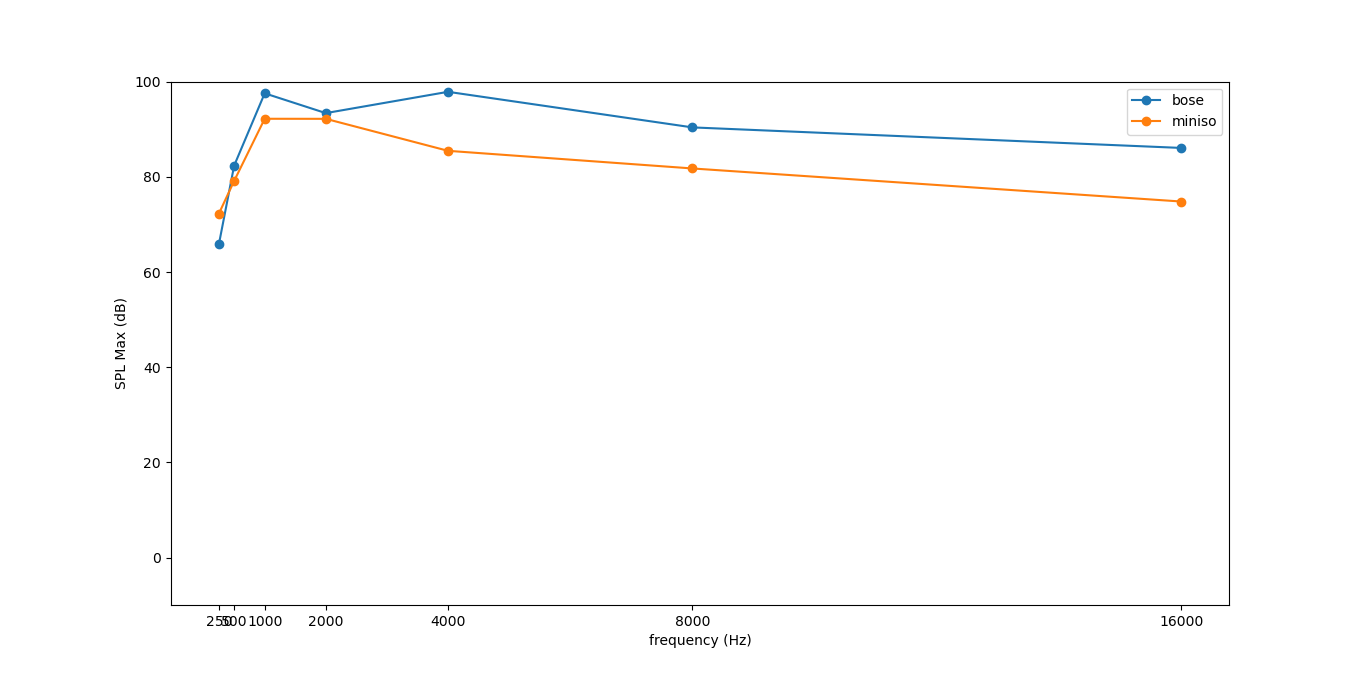
\includegraphics[width=450pt]{images/graph/all_allmax}
		\caption{Komparasi level maximum kedua headphone}
	\end{figure}
\end{document}